
\SetKwFunction{FDPTimelinesCosts}{DPTimelinesCosts}
\subsection{QPTAS for the $T||V,c||C_{max}$ problem}

The following algorithh is a simplified version of the QPTAS provided in \cite{dereniowski2017ApproxSsForGeneralBSinWTs}. The core idea of the algorithm is the same, however, our solution uses the language of decision trees instead of the language of sequence assignments, which makes the algorithm more intuitive.

For the rest of the analysis, without loss of the generality, we will assume that $T$ is rooted in a vertex $v$ minimizing $c\br{v}$.  We will also assume that all costs are normalized, so that $\max_{v\in V\br{T}}\brc{c\br{v}}=1$. If not, the costs are scaled by dividing them by $\max_{v\in V\br{T}}\brc{c(v)}$. Note that this operation does not affect the optimality of a strategy or the quality of an approximation.
\begin{observation}\label{basicBoundsOnCost}
    Let $T$ be a tree such that $\spr{V\br{T}}> 1$ and $c:V\to \mathbb{R}^+$ be a normalized weight function. Then, $1\leq \OPT(T) \leq \fl{\log n}+1$.
    \begin{proof}
        The first inequality is due to the fact that there exists $v\in V\br{T}$, such that $c\br{v}=1$ and for any decision tree $D$ we have $v\in Q_{D}\br{T,v}$. The second inequality is due to the fact that we can always locate the target using $\fl{\log n}+1$ queries \cite{OnakParys2006GenOfBSSInTsAndFLikePosets}.
    \end{proof}
\end{observation}
\subsubsection{Rounding}
We will use the following rounding schem which will allow us to discretise the space of possible solutions to process it efficiently. Let $p \in\mathbb{N}$, and $k=a/pn$ for some $a\in\mathbb{N}$. Define:
$$
c'\br{v}=\begin{cases}
    \cl{c\br{c}}_k, & \text{if } c\br{v}>pk, \text{ in which case the vertex will be called \textit{heavy}},\\
    \cl{c\br{c}}_{\frac{1}{pn}}, & \text{otherwise, in which case the vertex will be called \textit{light}}.\\
\end{cases}
$$

\begin{lemma}\label{rounded_dt_lemma}
    $$
    \OPT\br{T,c'}\leq \br{1+\frac{2}{p}}\cdot \OPT\br{T,c}
    $$
    \begin{proof}
        Let $D^*$ be an optimal strategy for $\br{T,c}$. By definition, we have that for every vertex $v\in V\br{T}$, $c'\br{v}\leq \br{1+\frac{1}{p}}\cdot c\br{v}+\frac{1}{p}n$ and therefore:
        \begin{align*}
            \OPT\br{T, c'}&\leq \COST_{D^*}\br{T,c'}=\max_{v\in V\br{T}}\brc{\sum_{q\in Q_{D^*}\br{T,v}}c'\br{q}}
            \\&
            \leq \max_{v\in V\br{T}}\brc{\sum_{q\in Q_{D^*}\br{T,v}}\br{\br{1+\frac{1}{p}}\cdot c\br{v}+\frac{1}{pn}}}
            \\&
            \leq \frac{1}{p}+\br{1+\frac{1}{p}}\cdot \max_{v\in V\br{T}}\brc{\sum_{q\in Q_{D^*}\br{T,v}}c\br{v} }\leq \br{1+\frac{2}{p}}\OPT\br{T,c}
        \end{align*}

        where in the third inequality we used the fact that for every $v\in V\br{T}$, $\spr{Q_{D^*}\br{T,v}}\leq n$ and in the last inequality we used Observation \ref{basicBoundsOnCost}.
    \end{proof}
\end{lemma}

While calculating the decision tree, we will divide the time into boxes of duration $k$, which will be further subdivided into $a$ identical slots of length $\frac{1}{pn}$. Let $t_q$ denote the start of some query in a decision tree $D$. Note that the numbers $t_v$ provide a complete information about any decision tree, and are an equiavalent representation of any strategy. We will assume that for any heavy vertex $v\in V\br{T}$, $t_v$ is an integer multiple of $c$ and for any light vertex $v\in V\br{T}$, $t_v$ is an integer multiple of $\frac{1}{pn}$. \footnote{Note that by doing so, we allow decision trees to contain idle time intervals, in which no queries are scheduled. However, if this occurs, after obtaining such decision tree, we simply delete the idle times, which results in a valid decision tree} We have the following lemma:
\begin{lemma}\label{aligned_dts_lemma}
    There exists a decision tree $D$ for $\br{T,c'}$, such that $\COST_{D}\br{T, c'}\leq \br{1+\frac{3}{p}}\cdot\OPT\br{T, c'}$ and for every vertex $v\in V\br{T}$ we have:
    \begin{enumerate}
        \item if $c\br{v}> pk$, then $t_v/k\in\mathbb{N}$ (every heavy query is aligned to a multiple of $c$),
        \item if $c\br{v}\leq pk$, then $t_vpn\in\mathbb{N}$ (every light query is aligned to a multiple of $\frac{1}{pn}$).
    \end{enumerate}
    \begin{proof}
        Let $D^*$ by any optimal decision tree for $\br{T,c'}$. For any $v\in V\br{T}$, let $t_v^*$ be the start of query to $v$ in $D^*$ and let $t_v'=\br{1+\frac{2}{p}}t_v^*$, thus construction a new decision tree $D'$. Since in this new decision tree $D'$, the ordering of vertices is exactly the same as in $D^*$, for any two consecutive queries $v,u$ in $D'$ we have:
        $$
            t_u'-t_v'=\br{1+\frac{2}{p}}\cdot\br{t_u-t_v}\geq \br{1+\frac{2}{p}}\cdot c\br{v}
        $$

        We now construct $D$ as follows: If $v\in V\br{T}$ is heavy, we assign $t_v=\cl{t_v'}_k$ and $t_v=t_v'$ otherwise. For any two consecutive queries $v,u$ in $D$, such that $v$ is heavy we have:
        $$
        t_u-\cl{t_v'}_k>t_u-t_v-k\geq \br{1+\frac{2}{p}}\cdot c\br{v}-k>w\br{v}+k>c'\br{v}
        $$

        So we conclude that no two queries overlap. To obtain the second part of the claim, we round up the starting time of each query to a light vertex in $D$ to an integer multiple of $\frac{1}{pn}$. We have:
        \begin{align*}
            \COST_{D}\br{T,c'}&
            \leq \max_{v\in V\br{T}}\brc{\sum_{q\in Q_{D^*}\br{T,v}}\br{\br{1+\frac{2}{p}}\cdot c'\br{v}+\frac{1}{pn}}}
            \\&
            \leq \frac{1}{p}+\br{1+\frac{2}{p}}\cdot \max_{v\in V\br{T}}\brc{\sum_{q\in Q_{D^*}\br{T,v}}c'\br{v} }\leq \br{1+\frac{3}{p}}\OPT\br{T,c'}
        \end{align*}

        where in the third inequality we used the fact that for every $v\in V\br{T}$, $\spr{Q_{D}\br{T,v}}\leq n$ and in the last inequality we used Observation \ref{basicBoundsOnCost}.
    \end{proof}
\end{lemma}

We will call a decision tree fulfilling above conditions \textit{aligned}. In subsequent considerations, we will focus ourselves of finding such decision trees, whose properties will allow us to devise an efficient dynamic programming procedure finding an optimal, aligned decision tree. 

\subsubsection{Heavy module contraction, up and down responses}
Since, our decision tree is rooted, we can reasonably talk about up and down responses to a query. An \textit{up} response to a query to $v$ in $T$ occurs when the connected component $\in T-v$, which is the reply happens to contain $r\br{T}$. If this is not the case, then such response is called a \textit{down} response. As it will turns out, a repeating occurance of light queries with down responses will become problematic for our algorithm. To account for this issue we will use the following notions:

We will define a new measure of cost for aligned deision trees called the \textit{aligned cost}. Let $D$ be any aligned strategy for $\br{t,c'}$. For any query $q\in V\br{D}$ and a vertex $v\in V\br{T}$, let the contribution $\kappa_{T,c,k}\br{q,v}$ be defined as:
$$
\kappa_{T,c}\br{q, v}= \begin{cases}
    0, & \text{if } c\br{v}\leq pk \text{ and the response to query $q$ in $T$, towards $v$ is down},\\
    c\br{q}, & \text{otherwise}.
\end{cases}
$$

Then, the \textit{aligned cost} of $D$ is defined as:

$$
\COST'_D\br{T,c',;}=\max_{v\in V\br{T}}\brc{\sum_{q\in Q_D\br{T,v}}\kappa_{T,c', k}\br{q,v}}.
$$

Let $\OPT'\br{T,c',k}$ denote the optimal aligned cost among all aligned decision trees for $\br{T,c',k}$.
The above cost, serves as a way to "ignore" all od the costs of light queries with down responses. Since of course, the amount of such queries may be of order $O\br{n}$, the difference between $\COST'_D\br{T,c',k}$ and $\COST_D\br{T,c',k}$ may grow almost arbitrarily large. However, we will make sure that this does not happen to often, which will give us the desired bound on the cost of the solution.


\begin{figure}[htbp]
    \begin{minipage}[t]{0.5\textwidth}
    \centering
    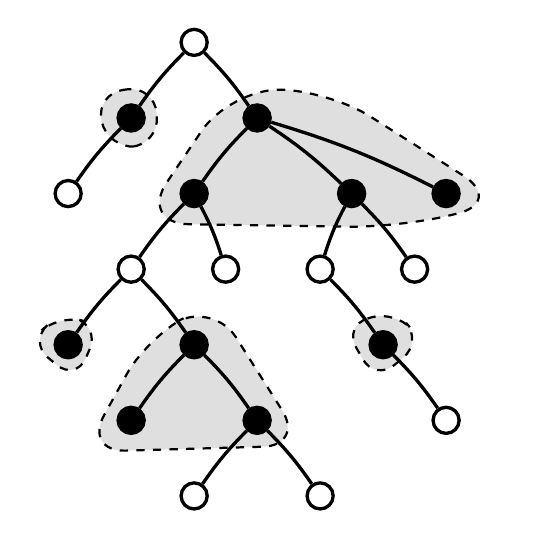
\begin{tikzpicture}[every node/.style={draw, very thick}, every path/.style={very thick}]
    
    \draw[dashed, thick, rounded corners = 10pt, fill= gray!25]
         (-1.25,5.75)  -- (-0.5,5.85)--  (-0.45,5.1) -- (-1.1,5.05) -- cycle;

    \draw[dashed, thick, rounded corners = 18pt, fill= gray!25]
        (0.45,5.8)  -- (1.7,5.8)-- (3.95,4.37) -- (2.6,4.05) -- (-0.7,4.1) -- cycle;
    \draw[dashed, thick, rounded corners = 9pt, fill= gray!25]
        (-2.1,2.6) -- (-1.7,2.95) -- (-1.2,2.8)  -- (-1.5,2.1) -- cycle;
        
    \draw[dashed, thick, rounded corners = 15pt, fill= gray!25]
         (-0.6,2.65) -- (0.25,3.1) -- (1.4,1.28) -- (-1.4,1.2) -- cycle;

    \draw[dashed, thick, rounded corners = 9pt, fill= gray!25]
        (1.9,2.8)  -- (2.55,3)  -- (2.9,2.6) -- (2.3,2.1) -- cycle;
    
    \node[circle, draw, fill=white] (1) at (0,6.4) {};
    
    \node[circle, draw, fill=black] (2) at (-0.8,5.44) {};
    \node[circle, draw, fill=black] (3) at (0.8,5.44) {};

    \node[circle, draw, fill=white] (4) at (-1.6,4.48) {};
    \node[circle, draw, fill=black] (5) at (0,4.48) {};
    \node[circle, draw, fill=black] (6) at (2.0,4.48) {};
    \node[circle, draw, fill=black] (7) at (3.2,4.48) {};
    
    \node[circle, draw, fill=white] (8) at (-0.8,3.52) {};
    \node[circle, draw, fill=white] (9) at (0.4,3.52) {};
    \node[circle, draw, fill=white] (10) at (1.6,3.52) {};
    \node[circle, draw, fill=white] (11) at (2.8,3.52) {};
    
    \node[circle, draw, fill=black] (12) at (-1.6,2.56) {};
    \node[circle, draw, fill=black] (13) at (0,2.56) {};
    \node[circle, draw, fill=black] (14) at (2.4,2.56) {};
    
    \node[circle, draw, fill=black] (15) at (-0.8,1.6) {};
    \node[circle, draw, fill=black] (16) at (0.8,1.6) {};
    \node[circle, draw, fill=white] (17) at (3.2,1.6) {};
    
    \node[circle, draw, fill=white] (18) at (0,0.64) {};
    \node[circle, draw, fill=white] (19) at (1.6,0.64) {};
    
    \draw[bend right=5] (1) to (2);
    \draw[bend left=5] (1) to (3);
    
    \draw[bend right=5] (2) to (4);
    \draw[bend right=5] (3) to (5);
    \draw[bend left=5] (3) to (6);
    \draw[bend left=5] (3) to (7);
    
    \draw[bend right=5] (5) to (8);
    \draw[bend left=5] (5) to (9);
    \draw[bend right=5] (6) to (10);
    \draw[bend left=5] (6) to (11);
    
    \draw[bend right=5] (8) to (12);
    \draw[bend left=5] (8) to (13);
    \draw[bend left=5] (10) to (14);
    
    \draw[bend right=5] (13) to (15);
    \draw[bend left=5] (13) to (16);
    \draw[bend left=5] (14) to (17);
    
    \draw[bend right=5] (16) to (18);
    \draw[bend left=5] (16) to (19);

    \end{tikzpicture}
\end{minipage}
    \begin{minipage}[t]{0.5\textwidth}
    \centering
    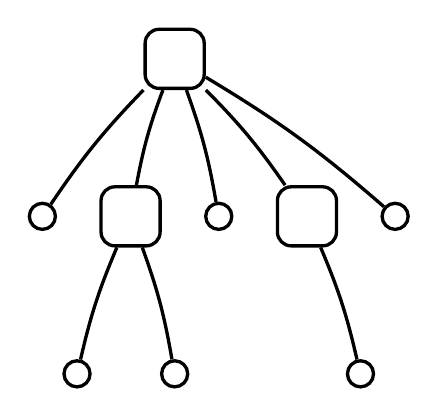
\begin{tikzpicture}[every node/.style={draw,rounded corners=5pt, very thick}, every path/.style={very thick}]
    
    \node[rectangle, minimum size=0.75cm, draw] (1) at (-0.56,10) {};
    
    \node[circle, draw] (2) at (-2.24,8) {};
    \node[rectangle, minimum size=0.75cm, draw] (3) at (-1.12,8) {};
    \node[circle, draw] (4) at (0,8) {};
    \node[rectangle, minimum size=0.75cm, draw] (5) at (1.12,8) {};
    \node[circle, draw] (6) at (2.24,8) {};
    
    \node[circle, draw] (7) at (-1.8,6) {};
    \node[circle, draw] (8) at (-0.56,6) {};
    \node[circle, draw] (9) at (1.8,6) {};
    
    \draw[bend right=5] (1) to (2);
    \draw[bend right=5] (1) to (3);
    \draw[bend left=5] (1) to (4);
    \draw[bend left=5] (1) to (5);
    \draw[bend left=5] (1) to (6);
    
    \draw[bend right=5] (3) to (7);
    \draw[bend left=5] (3) to (8);
    \draw[bend left=5] (5) to (9);

    \end{tikzpicture}
\end{minipage}
    \caption[Heavy module contraction]{Example of contracting 5 heavy modules. Black vertices represent heavy vertices, white vertices represent light vertices and square vertices represent vertices which were a parent of at least one heavy module before contraction.}\label{exampleHeavymoduleContraction}
\end{figure}
We define a \textit{heavy module} as $H\subseteq V\br{T}$ such that: $T[H]$ is connected, every $v \in H$ is heavy, i. e., $c\br{v}\geq pk$ and $H$ is maximal - no vertex can be added to it without violating one of its properties. A \textit{contraction} of a heavy module $H$ is an operation which consists of deleting all of the vertices in $H$ from $T$ and connecting every vertex $u$ which was a child of some vertex in $H$ to the parent of $r\br{T\angl{H}}$ if it exists. For example see Figure \ref{exampleHeavymoduleContraction}.

\subsubsection{The main procedure}

We will use the following proposition about the existence of the \FBuildDT procedure:
\begin{proposition}\label{BuildDTPropodisition}
     Let $T$ be a tree, $c:V\br{T}\to \mathbb{R}_{>0}$ $D_C$ a decision tree for $T$ with all heavy groups contracted, $p\in \mathbb{N}$ be a constant, $k\in \mathbb{R}_{>0}$ be the box size and $d\in \mathbb{N}$ be maximal depth. There exists a \FBuildDT procedure which:
     \begin{enumerate}
        \item Either determines that $kd\leq \OPT'\br{T, c',k}$ and returns an aligned decision tree $D$, such that:
        $$
            \COST_{D}\br{T,c',k}=\OPT'\br{T,c',k}+\COST_{D_C}\br{T,c'}.
        $$
        \item Or determines that $kd > \OPT'\br{T, c',k}$ and such decision tree does not exist.
        \item The procedure runs in $\br{pn}^d$ time.
     \end{enumerate}
\end{proposition}
The proof will be provided in the next section.
We will now prove the Proposition \ref{QPTAS}.


\begin{algorithm}
\caption{The QPTAS for $T||V,c,w||C_{max}$.}\label{qptas_pseudocode}
\SetKwProg{Fn}{Procedure}{:}{}
\Fn{$\FQPTAS\br{T,c,\epsilon}$}{
    $p\gets\cl{24/\epsilon}$,
    $k\gets 0$,
    $D\gets \emptyset$.

    $d\gets p^2\cdot\br{\fl{\log\br{n}}+1}$.

    \Repeat{$D \neq \emptyset$}
    {
        $k\gets k+\frac{1}{pn}$.

        \ForEach{$v\in V\br{T}$}{
            \If{$c\br{v}>pk$}{
                $c'\br{v}\gets \cl{c\br{v}}_k$.
            }
            \Else{
                $c'\br{v}\gets \cl{c\br{v}}_{\frac{1}{pn}}$.
            }
            
        }

        $T_C\gets T$ with all heavy modules contracted.

        $D_C\gets\FRankingBasedDT\br{T_C}$.

        $D\gets \FBuildDT\br{T, c', D_C, p, k, d}$.
    }   
    \Return $D$.
    
}
\end{algorithm}

The Algorithm \ref{qptas_pseudocode} starts by picking $p=\cl{\frac{24}{\epsilon}}$ and assigning $k=0$ and $d=p^2\cdot\br{\fl{\log n}+1}$. At each iteration of the repeat loop, the algorithm picks $k$ to be the next 
integer multiple of $\frac{1}{pn}$, performs the rounding operation introduced above, creates a decision tree $D_C$ for tree $T$ with all heavy modules contracted and tries to create decision tree $D$, by applying Proposition \ref{BuildDTPropodisition}. Once the \FBuildDt procedure returns a non-empty solution, the \FQPTAS procedure terminates and returns the constructed decision tree $D$. Let $k'$ be the value of $k$ for which $D$ was found. Since we know that $k'\leq \frac{\OPT'\br{T,c',k'}}{d}=\frac{\OPT'\br{T,c'}}{p^2\cdot\br{\fl{\log n}+1}}$, we have that:
\begin{align*}
    \COST_{D}\br{T,c'}&\leq \OPT'\br{T,c'}+pc'\cdot \br{\fl{\log n}+1}\leq \OPT'\br{T,c'}+p\cdot \br{p^2\cdot\br{\fl{\log n}+1}}\cdot \frac{\OPT'\br{T,c'}}{\fl{\log n}+1} \\
    & \leq \br{1+\frac{1}{p}}\cdot\OPT'\br{T,c'}\leq \br{1+\frac{1}{p}}\cdot\br{1+\frac{2}{p}}\cdot\br{1+\frac{3}{p}}\cdot\OPT\br{T,c}
    \\&
    \leq \br{1+\frac{24}{p}}\cdot\OPT\br{T,c} = \br{1+\frac{24}{\cl{\frac{24}{\epsilon}}}}\cdot\OPT\br{T,c}\leq \br{1+\epsilon}\cdot \OPT\br{T,c}
\end{align*}
    
where the second inequality is by applying Corollary \ref{vertexRankingCorollary} and the fourth inequality is by Lemma \ref{rounded_dt_lemma} and Lemma \ref{aligned_dts_lemma}.

We can assume that $c=\text{poly}\br{n}$, since beyond that the problem can be solved to optimality in $O\br{2^nn}$ time. Therefore the running time of the procedure is bounded by:
$$
n^{O\br{d}}=n^{O\br{p^2\log n}}=n^{O\br{\log n/\epsilon^2}}.
$$
\subsubsection{Medusa tree construction}


\SetKwFunction{FDPTimelines}{DPTimelines}
\begin{figure}[htp]
\begin{minipage}[t]{1\textwidth}
    \centering
    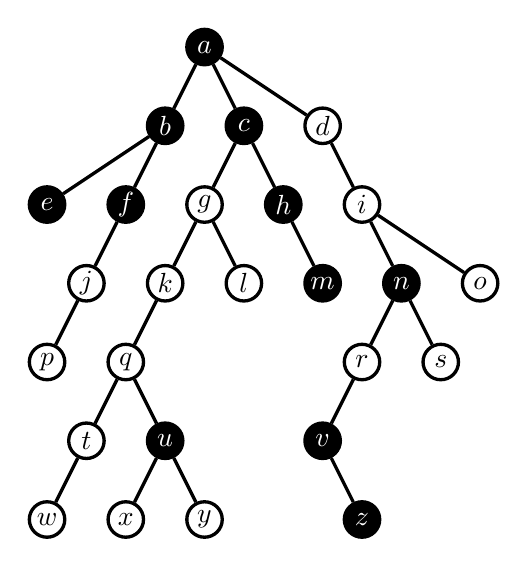
\begin{tikzpicture}[every path/.style={very thick}]
    
    \node[text=white, circle, draw, minimum size=0.45cm, inner sep=0pt, fill=black] (1) at (0,0) {$a$};

    \node[text=white, circle, draw, minimum size=0.45cm, inner sep=0pt, fill=black] (2) at (-0.5,-1) {$b$};

    \node[text=white, circle, draw, minimum size=0.45cm, inner sep=0pt, fill=black] (3) at (0.5,-1) {$c$};

    \node[circle, draw, minimum size=0.45cm, inner sep=0pt, fill=white] (4) at (1.5,-1) {$d$};

    \draw[] (1) to (2);
    \draw[] (1) to (3);
    \draw[] (1) to (4);

    \node[text=white, circle, draw, minimum size=0.45cm, inner sep=0pt, fill=black] (5) at (-2,-2) {$e$};

    \node[text=white, circle, draw, minimum size=0.45cm, inner sep=0pt, fill=black] (6) at (-1,-2) {$f$};

    \node[circle, draw, minimum size=0.45cm, inner sep=0pt, fill=white] (7) at (0,-2) {$g$};

    \node[text=white, circle, draw, minimum size=0.45cm, inner sep=0pt, fill=black] (8) at (1,-2) {$h$};

    \node[circle, draw, minimum size=0.45cm, inner sep=0pt, fill=white] (9) at (2,-2) {$i$};

    \draw[] (2) to (5);
    \draw[] (2) to (6);

    \draw[] (3) to (7);
    \draw[] (3) to (8);

    \draw[] (4) to (9);

    \node[circle, draw, minimum size=0.45cm, inner sep=0pt, fill=white] (10) at (-1.5,-3) {$j$};

    \node[circle, draw, minimum size=0.45cm, inner sep=0pt, fill=white] (11) at (-0.5,-3) {$k$};

    \node[circle, draw, minimum size=0.45cm, inner sep=0pt, fill=white] (12) at (0.5,-3) {$l$};

    \node[text=white, circle, draw, minimum size=0.45cm, inner sep=0pt, fill=black] (13) at (1.5,-3) {$m$};

    \node[text=white, circle, draw, minimum size=0.45cm, inner sep=0pt, fill=black] (14) at (2.5,-3) {$n$};

    \node[circle, draw, minimum size=0.45cm, inner sep=0pt, fill=white] (15) at (3.5,-3) {$o$};

    \draw[] (6) to (10);

    \draw[] (7) to (11);
    \draw[] (7) to (12);

    \draw[] (8) to (13);

    \draw[] (9) to (14);
    \draw[] (9) to (15);

    \node[circle, draw, minimum size=0.45cm, inner sep=0pt, fill=white] (16) at (-2,-4) {$p$};

    \node[circle, draw, minimum size=0.45cm, inner sep=0pt, fill=white] (17) at (-1,-4) {$q$};

    \node[circle, draw, minimum size=0.45cm, inner sep=0pt, fill=white] (18) at (2,-4) {$r$};

    \node[circle, draw, minimum size=0.45cm, inner sep=0pt, fill=white] (19) at (3,-4) {$s$};

    \draw[] (10) to (16);
    
    \draw[] (11) to (17);
    
    \draw[] (14) to (18);
    \draw[] (14) to (19);

    \node[circle, draw, minimum size=0.45cm, inner sep=0pt, fill=white] (20) at (-1.5,-5) {$t$};

    \node[text=white, circle, draw, minimum size=0.45cm, inner sep=0pt, fill=black] (21) at (-0.5,-5) {$u$};

    \node[text=white, circle, draw, minimum size=0.45cm, inner sep=0pt, fill=black] (22) at (1.5,-5) {$v$};

    \draw[] (17) to (20);
    \draw[] (17) to (21);

    \draw[] (18) to (22);


    \node[circle, draw, minimum size=0.45cm, inner sep=0pt, fill=white] (23) at (-2,-6) {$w$};

    \node[circle, draw, minimum size=0.45cm, inner sep=0pt, fill=white] (24) at (-1,-6) {$x$};

    \node[circle, draw, minimum size=0.45cm, inner sep=0pt, fill=white] (25) at (0,-6) {$y$};

    \node[text=white, circle, draw, minimum size=0.45cm, inner sep=0pt, fill=black] (26) at (2,-6) {$z$};

    
    \draw[] (20) to (23);

    \draw[] (21) to (24);
    \draw[] (21) to (25);

    \draw[] (22) to (26);
    
    \end{tikzpicture}
    \caption[Input tree $T$ with a heavy root]{}\label{tree_h_root}
\end{minipage}
\begin{minipage}[t]{0.49\textwidth}
    \centering
    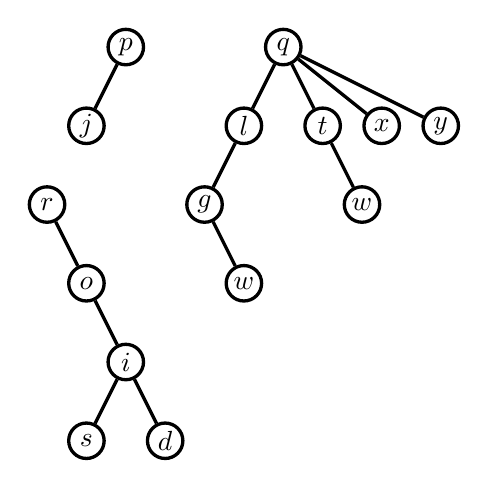
\begin{tikzpicture}[every path/.style={very thick}]
    
    \node[circle, draw, minimum size=0.45cm, inner sep=0pt, fill=white] (1) at (0,0) {$p$};

    \node[circle, draw, minimum size=0.45cm, inner sep=0pt, fill=white] (2) at (-0.5,-1) {$j$};

    \draw[] (1) to (2);

    \node[circle, draw, minimum size=0.45cm, inner sep=0pt, fill=white] (3) at (2,0) {$q$};



    \node[circle, draw, minimum size=0.45cm, inner sep=0pt, fill=white] (4) at (1.5,-1) {$l$};

    \node[circle, draw, minimum size=0.45cm, inner sep=0pt, fill=white] (5) at (2.5,-1) {$t$};

    \node[circle, draw, minimum size=0.45cm, inner sep=0pt, fill=white] (6) at (3.25,-1) {$x$};

    \node[circle, draw, minimum size=0.45cm, inner sep=0pt, fill=white] (7) at (4,-1) {$y$};

    

    \draw[] (3) to (4);
    \draw[] (3) to (5);
    \draw[] (3) to (6);
    \draw[] (3) to (7);

    \node[circle, draw, minimum size=0.45cm, inner sep=0pt, fill=white] (8) at (1,-2) {$g$};

    \node[circle, draw, minimum size=0.45cm, inner sep=0pt, fill=white] (9) at (3,-2) {$w$};

    \draw[] (4) to (8);
    \draw[] (5) to (9);

    \node[circle, draw, minimum size=0.45cm, inner sep=0pt, fill=white] (10) at (1.5,-3) {$w$};

    \draw[] (8) to (10);



    \node[circle, draw, minimum size=0.45cm, inner sep=0pt, fill=white] (11) at (-1,-2) {$r$};


    \node[circle, draw, minimum size=0.45cm, inner sep=0pt, fill=white] (12) at (-0.5,-3) {$o$};

    \draw[] (11) to (12);

    \node[circle, draw, minimum size=0.45cm, inner sep=0pt, fill=white] (13) at (0,-4) {$i$};

    \draw[] (12) to (13);

    \node[circle, draw, minimum size=0.45cm, inner sep=0pt, fill=white] (14) at (-0.5,-5) {$s$};

    \node[circle, draw, minimum size=0.45cm, inner sep=0pt, fill=white] (15) at (0.5,-5) {$d$};

    \draw[] (13) to (14);
    \draw[] (13) to (15);


    
    \end{tikzpicture}
    \caption[Input forest of decision trees for light vertices $F_C$.]{}\label{input_forest}
\end{minipage}
\begin{minipage}[t]{0.49\textwidth}
    \centering
    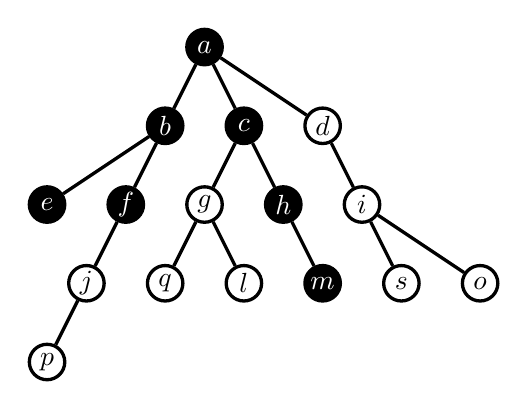
\begin{tikzpicture}[every path/.style={very thick}]
    
    \node[text=white, circle, draw, minimum size=0.45cm, inner sep=0pt, fill=black] (1) at (0,0) {$a$};

    \node[text=white, circle, draw, minimum size=0.45cm, inner sep=0pt, fill=black] (2) at (-0.5,-1) {$b$};

    \node[text=white, circle, draw, minimum size=0.45cm, inner sep=0pt, fill=black] (3) at (0.5,-1) {$c$};

    \node[circle, draw, minimum size=0.45cm, inner sep=0pt, fill=white] (4) at (1.5,-1) {$d$};

    \draw[] (1) to (2);
    \draw[] (1) to (3);
    \draw[] (1) to (4);

    \node[text=white, circle, draw, minimum size=0.45cm, inner sep=0pt, fill=black] (5) at (-2,-2) {$e$};

    \node[text=white, circle, draw, minimum size=0.45cm, inner sep=0pt, fill=black] (6) at (-1,-2) {$f$};

    \node[circle, draw, minimum size=0.45cm, inner sep=0pt, fill=white] (7) at (0,-2) {$g$};

    \node[text=white, circle, draw, minimum size=0.45cm, inner sep=0pt, fill=black] (8) at (1,-2) {$h$};

    \node[circle, draw, minimum size=0.45cm, inner sep=0pt, fill=white] (9) at (2,-2) {$i$};

    \draw[] (2) to (5);
    \draw[] (2) to (6);

    \draw[] (3) to (7);
    \draw[] (3) to (8);

    \draw[] (4) to (9);

    \node[circle, draw, minimum size=0.45cm, inner sep=0pt, fill=white] (10) at (-1.5,-3) {$j$};

    \node[circle, draw, minimum size=0.45cm, inner sep=0pt, fill=white] (11) at (-0.5,-3) {$q$};

    \node[circle, draw, minimum size=0.45cm, inner sep=0pt, fill=white] (12) at (0.5,-3) {$l$};

    \node[text=white, circle, draw, minimum size=0.45cm, inner sep=0pt, fill=black] (13) at (1.5,-3) {$m$};

    \node[circle, draw, minimum size=0.45cm, inner sep=0pt, fill=white] (14) at (2.5,-3) {$s$};

    \node[circle, draw, minimum size=0.45cm, inner sep=0pt, fill=white] (15) at (3.5,-3) {$o$};

    \draw[] (6) to (10);

    \draw[] (7) to (11);
    \draw[] (7) to (12);

    \draw[] (8) to (13);

    \draw[] (9) to (14);
    \draw[] (9) to (15);

    \node[circle, draw, minimum size=0.45cm, inner sep=0pt, fill=white] (16) at (-2,-4) {$p$};


    \draw[] (10) to (16);

    
    \end{tikzpicture}
    \caption[Medusa tree $T_M$]{}\label{medusa_tree}
\end{minipage}
\caption[Construction of the medusa tree]{Construction of the medusa tree. Figure \ref{tree_h_root} shows example input tree $T$ with a heavy root. Figure \ref{input_forest} shows example input forest of decision trees for light vertices $F_C$. Figure \ref{medusa_tree} shows the constructed medusa tree $T_M$.}\label{medusa_tree_construction_figure}
\end{figure}

\begin{algorithm}
\caption{The \FBuildDT procedure ($p, k$, and $d$ are global parameters).}\label{buildDTpseudocode}
\SetKwProg{Fn}{Procedure}{:}{}
\Fn{$\FBuildDT\br{T, c, F_C}$}{
    \If{$c\br{r\br{T}}>pc$}{
        $D\gets\br{\brc{r\br{F_C}}, \emptyset}$.

        \ForEach{\textnormal{$T'\in T-r\br{D}$ and forest $F'_C\in D-r\br{D}$, such that $V\br{F'_C} = V\br{T'}$}}{
            $D'\gets\FBuildDT\br{T', c, F'_C}$.

            Hang $D'$ in $D$ below $r\br{D}$.
        }

    }
    \Else{
        $H\gets \brc{v\in V\br{T}|c\br{v} > pk \text{ and for every ancestor $u$ of $v$}, c\br{u}> pk}$.

        $L\gets \brc{v\in V\br{T}|c\br{c}\leq pk}$. 

        \ForEach{\textnormal{$v\in V\br{F_C}$ and ancestor $u$ of $v$ in $F_C$}}
        {
            \If{\textnormal{$v$ is an ancestor of $u$ in $T$}}
            {
                $L$\gets $L - u$
            }
        }
        
        $V_M\gets L\cup H$.

        $M\gets \br{V_M, \brc{uv|u,v\in V_M, \mathcal{P}_{u,v}\cap V_M=\emptyset}}$.

        $\mathcal{A}\gets$ dictionary, such that for each $v\in V_M$, $\mathcal{A}[v]\gets \emptyset$.

        \ForEach{\textnormal{$T'\in T-V_M$ and forest $F'_C\in D-V_M$, such that $V\br{F'_C} = V\br{T'}$}}
        {
            $D'\gets \FBuildDT\br{T',c, D'_C}$.

            $\mathcal{A}[p]\gets \mathcal{A}[p] \cup \brc{D'}$.
        }

        $D\gets \FDPTimelinesCosts\br{M, c}$.

    }
    \Return $D$.
}
\end{algorithm}


\subsubsection{Dynamic programming procedure for fixed box size}



